\subsection{Basic Oceanographic Equations}

The Coriolis parameter $f$ is given by
\begin{equation}
f=2 \Omega \sin \varphi,
\label{eq:coriolis}
\end{equation}
where $\varphi$ is the latitude of the position and $\Omega$ is the angular
 frequency of the Earth's rotation.

\subsubsection{Basic Fluid Mechanics}
Fluid mechanics is based on three simple equations~\cite{landau1959course}:
 The conservation of matter,
\begin{equation}
\frac{\partial \rho}{\partial t} + \boldsymbol{\nabla}(\rho \boldsymbol{u}) = 0,
\tag{Matter}
\label{eq:Matter}
\end{equation}
the conservation of momentum,
\begin{equation}
\rho\left (\frac{\partial \mathbf{u}}{\partial t}
+ \mathbf{u}(\boldsymbol{\nabla}\cdot \mathbf{u})\right) =
- \boldsymbol{\nabla}P + \boldsymbol{\nabla}\cdot \underline{\underline{\tau}}
- \rho\boldsymbol{\nabla}\phi,
\tag{Momentum}
\end{equation}
and the conservation of energy,
\begin{equation}
\begin{array}{l}
\rho \left( \frac{\partial h}{\partial t} + \boldsymbol{\nabla}
\cdot (h\mathbf{u})\right) = \\ \quad\quad- \left( \frac{\partial P}{\partial t}
+ \mathbf{u}\cdot (\boldsymbol{\nabla} P) \right)
+ \boldsymbol{\nabla}\cdot (k \boldsymbol{\nabla} T )
+ (\underline{\underline{\tau}}\cdot\boldsymbol{\nabla})\mathbf{u}.\end{array}
\tag{Energy}
\end{equation}
Where we have assumed that we are in an inertial frame and the variables are
labelled as in Table~\ref{tab:fluid_variables}.

\begin{table}[h!]
    \centering
    \begin{tabular}{ll}
        $\rho$ & Density. \\
        $t$ & Time. \\
        $\mathbf{u}$ & Velocity. \\
        $P$ & Pressure. \\
        $\underline{\underline{\tau}}$ & Deviatronic stress (2nd order tensor). \\
        $\phi$ & Gravitational potential. \\
         $h$ & Enthalpy.\\
         $T$ & Temperature. \\
         $k$ & Thermal conductivity.\\
         $c_p$ & Heat capacity.\\
         $\eta$ & Viscosity. \\
         $H$ & Heat production density.\\
    \end{tabular}
    \caption{Symbols for fluid mechanical equations.}
    \label{tab:fluid_variables}
\end{table}

\subsubsection{Boussenesq Approximation}
We can also normally assume that all density variations can be ignored that
 are not on the gravitational term (the Boussenesq approximation),
  which simplifies the equations considerably as Equation~\ref{eq:Matter} becomes
\begin{equation}
    \boldsymbol{\nabla}\cdot\mathbf{u} = 0, \tag{B-Matter}
\end{equation}
and we also could derive that
\begin{equation}
\rho\left (\frac{\partial \mathbf{u}}{\partial t}
+ \mathbf{u}(\boldsymbol{\nabla}\cdot \mathbf{u})\right)=
-\nabla P+\eta \nabla^{2} \mathbf{u}-\rho \boldsymbol{\nabla}\phi, \tag{B-Momentum}
\end{equation}
\begin{equation}
\rho c_{p}\left(\frac{\partial T}{\partial t}
+\mathbf{u} \cdot \nabla T\right)=k \nabla^{2} T+\rho H. \tag{B-Energy}
\end{equation}

\subsubsection{Extension to a Rotating Sphere}
\label{app:rotating_equations}
However the surface of the Earth reference frames rotate,
 which makes these equations less elegant.
  The final form of the equations in an earth bound reference frame
  is found by applying the identity
\begin{equation}
\frac{\mathrm{d}}{\mathrm{d} t} \boldsymbol{A}=
\left[\left(\frac{\mathrm{d}}{\mathrm{d} t}\right)_{r}
+\mathbf{\Omega} \times\right] \boldsymbol{A},
\end{equation}
for converting to a rotating reference frame to the previous equations.
\begin{equation}
\begin{array}{l}
\rho \frac{D \mathbf{u}}{D t}=\\\quad\quad-\boldsymbol{\nabla} P+
\eta \nabla^{2} \mathbf{u}+\frac{1}{3} \eta \nabla(\nabla \cdot \mathbf{u})
+\rho \mathbf{g}\\\quad\quad-\rho\left(2 \mathbf{\Omega} \times \mathbf{u}
+\mathbf{\Omega} \times(\mathbf{\Omega} \times \mathbf{x})
+\frac{d \mathbf{u}}{d t}\right)\end{array}.
\tag{R-Momentum}
\end{equation}

\subsubsection{The Ekman Spiral}

Due to the effects introduced in \cref{app:rotating_equations},
the wind does not simply cause the water to go in
the same direction~\cite{ekman1905influence}.
Instead, in the northern Hemisphere,
 the surface travels c.~45 degrees to the
right of the prevailing wind, and each subsequent
layer of the water travels to the right of that.
If the water column is deep enough, with
assumptions about the friction coefficients of the water column,
the net transport is 90 degrees to the right of the prevailing wind
(see Figure~\ref{fig:ekman}).\footnote{\url{https://oceanservice.noaa.gov/education/kits/currents/media/supp_cur05e.html}}

\begin{figure}
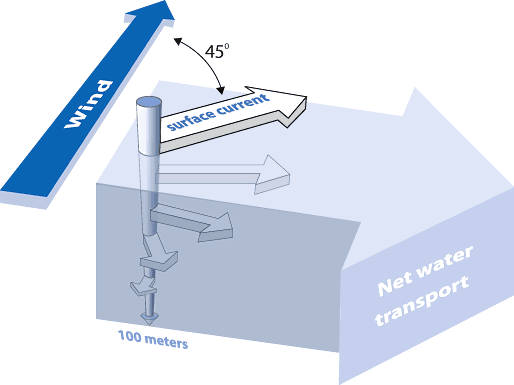
\includegraphics[width=\linewidth]{images/ekman_spiral.png}
\caption{The Ekman spiral.}
\label{fig:ekman}
\end{figure}
